\subsection{一次方程组的应用}\label{subsec:5-6}

对于某些含有两个或两个以上未知数的问题, 有时可以用一次方程组来求解。 下面我们来看几个例子。

\liti 某水利工地派 48 人去挖土和运土。 如果每人每天平均挖土 5 方或运土 3 方,
那么应怎样分配挖土和运土的人数, 正好能够使挖出的土及时运走?

分析: 这个问题里有两个未知数 —— 挖土人数和运土人数。未知数与已知数之间有以下的相等关系:

(1) 挖土人数 $+$ 运土人数 $=$ 派出的总人数;

(2) 每天挖土的总方数 $=$ 每天运土的总方数, 即 $5 \times (\text{挖土人数}) = 3 \times (\text{运土人数})$。

如果分别用 $x$, $y$ 表示挖土人数和运土人数, 那么根据上述相等关系, 就可以列出一个二元一次方程组。

\jie 设应分配 $x$ 人挖土, $y$ 人运土, 根据题意, 得\jiange
\begin{numcases}{}
    x + y = 48 \douhao \tag{1} \\
    5x = 3y    \juhao  \tag{2}
\end{numcases}

由 (2) 得,
\begin{gather*}
    x = \dfrac{3}{5}y \juhao \tag{3}
\end{gather*}

把 (3) 代入 (1),得
\begin{gather*}
    \dfrac{3}{5}y + y = 48 , \\
    8y = 240,
\end{gather*}

\fengeSuoyi{y = 30 \juhao}

把 $y = 30$ 代入 (3),得
$$ x = 18\juhao $$

\fengeSuoyi{\begin{cases} x = 18 \douhao \\ y = 30 \juhao \end{cases}}

答: 应分配 18 人挖土, 30 人运土。

\liti 运往某地两批物资, 第一批 360 吨, 用 6 节火车车皮加上 15 辆汽车正好装完;
第二批 440 吨,用 8 节火车车皮加上 10 辆汽车正好装完。 求每节火车车皮和每辆汽车平均各装多少吨。

分析: 这个问题有两个未知数 —— 每节火车车皮和每辆汽车平均所装货物的吨数。
未知数与已知数之间有以下的相等关系:

(1) $6 \times \text{(每节火车车皮平均装货的吨数)} + 15 \times \text{(每辆汽车平均装货的吨数)} = 360$;

(2) $8 \times \text{(每节火车车皮平均装货的吨数)} + 10 \times \text{(每辆汽车平均装货的吨数)} = 440$。

如果分别用 $x$,$y$ 表示每节火车车皮和每辆汽车平均装货的吨数, 那么根据上述相等关系, 就可以列出一个二元一次方程组。

解: 设每节火车车皮平均装货 $x$ 吨, 每辆汽车平均装货 $y$ 吨, 根据题意, 得\jiange
\begin{numcases}{}
    6x + 15y = 360 \douhao \tag{1} \\
    8x + 10y = 440 \juhao  \tag{2}
\end{numcases}

$(2) \times \dfrac{1}{2} - (1) \times \dfrac{1}{3}$,得
$$ 2x = 100 \douhao $$

\fengeSuoyi{x = 50 \juhao}

把 $x = 50$ 代入 (2),得
\begin{gather*}
    8 \times 50 + 10y = 440 \douhao \\
    10y = 40 \douhao
\end{gather*}

\fengeSuoyi{y = 4 \juhao}

\fengeSuoyi{\begin{cases} x = 50 \douhao \\ y = 4 \juhao \end{cases}}

答: 每节火车车皮平均装货 50 吨, 每辆汽车平均装货 4 吨。


\liti 用库存化肥给麦田追肥, 如果每公顷施 90 千克, 就缺少 3000 千克;
如果每公顷施 75 千克, 就剩余 4500 千克。 有多少公顷麦田? 库存化肥有多少千克?

分析: 这个问题里有两个未知数 —— 麦田的公顷数和库存化肥的千克数。
如果分别用 $x$,$y$ 表示这两个未知数, 那么未知数与已知数之间的关系如图 \ref{fig:5-2} 所示。

\begin{figure}[htbp]
    \centering
    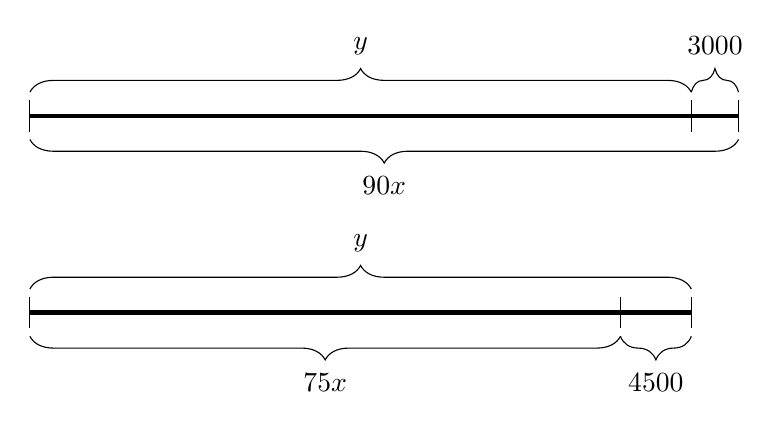
\begin{tikzpicture}
    \begin{scope}
        \pgfmathsetmacro{\a}{0}
        \pgfmathsetmacro{\b}{4.2*2}
        \pgfmathsetmacro{\c}{4.5*2}

        \draw [ultra thick] (\a, 0) -- (\c, 0);
        \foreach \x in {\a, \b, \c} {
            \draw (\x, 0.2) -- (\x, -0.2);
        }
        \draw[decorate, decoration={brace, amplitude=0.3cm}] (\a, 0.3) -- (\b, 0.3)
            node [pos=0.5, above=1em, align=center] {$y$};
        \draw[decorate, decoration={brace, amplitude=0.3cm}] (\b, 0.3) -- (\c, 0.3)
            node [pos=0.5, above=1em, align=center] {$3000$};
        \draw[decorate, decoration={brace,mirror, amplitude=0.3cm}] (\a, -0.3) -- (\c, -0.3)
            node [pos=0.5, below=1em, align=center] {$90x$};
    \end{scope}

    \begin{scope}[yshift=-2.5cm]
        \pgfmathsetmacro{\a}{0}
        \pgfmathsetmacro{\b}{3.75*2}
        \pgfmathsetmacro{\c}{4.2*2}

        \draw [ultra thick] (\a, 0) -- (\c, 0);
        \foreach \x in {\a, \b, \c} {
            \draw (\x, 0.2) -- (\x, -0.2);
        }
        \draw[decorate, decoration={brace, amplitude=0.3cm}] (\a, 0.3) -- (\c, 0.3)
            node [pos=0.5, above=1em, align=center] {$y$};
        \draw[decorate, decoration={brace,mirror, amplitude=0.3cm}] (\a, -0.3) -- (\b, -0.3)
            node [pos=0.5, below=1em, align=center] {$75x$};
        \draw[decorate, decoration={brace,mirror, amplitude=0.3cm}] (\b, -0.3) -- (\c, -0.3)
            node [pos=0.5, below=1em, align=center] {$4500$};
    \end{scope}
\end{tikzpicture}

    \caption{}\label{fig:5-2}
\end{figure}

解: 设有麦田 $x$ 公顷, 库存的化肥有 $y$ 千克, 根据题意, 得\jiange
\begin{numcases}{}
    90x = y + 3000 \douhao \tag{1} \\
    75x = y - 4500 \juhao  \tag{2}
\end{numcases}

$(1) - (2)$,得
\begin{gather*}
    15x = 7500 \douhao \\
    x = 500 \juhao
\end{gather*}

把 $x = 500$ 代入 (1),得
$$ 90 \times 500 = y + 3000 \juhao $$

\fengeSuoyi{y = 42000 \juhao}

\fengeSuoyi{\begin{cases} x = 500 \douhao \\ y = 42000 \juhao \end{cases}}

答: 有麦田 500 公顷, 库存化肥有 42000 千克。

\lianxi

列出一次方程组解下列应用题:

\begin{xiaotis}

\xiaoti{用大小两台拖拉机耕地, 一小时共耕了 2 公顷地。已知大拖拉机的效率是小拖拉机的 1.5 倍, 求大小拖拉机各耕了多少公顷地。}

\xiaoti{某间有 28 名工人, 生产一种螺栓和螺母, 每人每天平均能生产螺栓 12 个或螺母 18 个。
    应分配多少人生产螺拴,多少人生产螺母,能够使生产出的螺栓和螺母刚好配套(一个螺栓套两个螺母)?
}

\xiaoti{伍分和貳分的硬币共 100 枚,值 3 元 2 角。 这两种硬币各有多少枚?}

\xiaoti{一条船的载重量是 520 吨, 货舱载货容积是 $2000\lfm$。 现在装运甲、乙两种货物,
    甲种货物每吨的体积是 $2 \lfm$, 乙种货物每吨的体积是 $8 \lfm$。
    这两种货物各装多少吨,才能最大限度地利用这条船的载重量及载货容积?
}

\xiaoti{某工厂接受一批农具的定货任务, 按计划天数进行生产,
    如果平均每天生产 20 件, 就比定货任务还少 100 件;
    如果平均每天生产 23 件, 就可超过定货任务 20 件。
    这批农具的定货任务是多少件? 原计划几天完成?
}

\xiaoti{汽车从甲地到乙地, 如果每小时行驶 45 千米,就要延误 $\dfrac{1}{2}$ 小时到达;
    如果每小时行驶 50 千米, 就可提前 $\dfrac{1}{2}$ 小时到达。
    求从甲地到乙地的路程及原计划行驶的时间。
}

\end{xiaotis}
\lianxijiange

\liti 用浓度为 $5\%$ 和 $53\%$ 的两种烧碱溶液混合配制成浓度为 $25\%$ 的烧碱液 300 千克, 需用这两种烧碱溶液各多少千克?

分析: 这个问题里有两个未知数 —— 浓度为 $5\%$ 的烧碱溶液的千克数和浓度为 $53\%$ 的烧碱溶液的千克数。
如果分别用 $x$,$y$ 来表示这两个未知数, 那么未知数与已知数之间的关系如下表所示:\jiange

\begin{tblr}{hlines,vlines,
    rows = {halign=c, valign=m},
}
    \diagbox[innerwidth=8em, height=4em]{重量}{浓度} & {$5\%$的\\ 烧碱溶液} & {$53\%$的\\ 烧碱溶液} & {混合成$25\%$\\ 的烧碱溶液} \\
    {烧碱溶液的重量\\(千克)}   & $x$            & $y$             & 300 \\
    {所含纯烧碱的重量\\(千克)} & $5\% \cdot x$  & $53\% \cdot y$  & $25\% \cdot 300$ \\
\end{tblr}\jiange

根据下面的相等关系, 可以列出一个二元一次方程组:

混合前烧碱溶液的重量 $=$ 混合后烧碱溶液的重量;

混合前溶液中所含纯烧碱的重量 $=$ 混合后溶液中所含纯烧碱的重量。

\jie 设需用 $5\%$ 的烧碱溶液 $x$ 千克, $53\%$ 的烧溶液 $y$ 千克,根据题意,得\jiange
\begin{numcases}{}
    x + y = 300 \douhao \tag{1} \\
    5\% \cdot x + 53\% \cdot y = 25\% \cdot 300 \juhao  \tag{2}
\end{numcases}

化简 (2),得
\begin{gather*}
    5x + 53y = 7500 \juhao \tag{3}
\end{gather*}

$(3) - (1) \times 5$,得
$$ 48y = 6000 \douhao $$

\fengeSuoyi{y = 125 \juhao}

把 $y = 125$ 代入 (1),得
$$ x + 125 = 300 \douhao $$

\fengeSuoyi{x = 175 \juhao}

\fengeSuoyi{\begin{cases} x = 175\douhao \\ y = 125 \juhao \end{cases}}

答: 需用浓度为 $5\%$ 的烧碱溶液 175 千克, $53\%$ 的烧碱溶液 125 千克。


\liti 在代数式 $px + q$ 中, 当 $x= 2$ 时,它的值是 $-1$; 当 $x = 3$ 时, 它的值是 1, 求 $p$, $q$ 的值。

分析:这里的未知数是 $p$, $q$。 把 $x = 2$ 及 $x = 3$ 代入 $px + q$, 分别得值 $-1$, 1 ,
这就得到一个关于 $p$, $q$ 的二元一次方程组。 解这个方程组,就可以求出 $p$, $q$ 的值。

\jie 根据题意,得
\begin{numcases}{}
    2p + q = -1 \douhao \tag{1} \\
    3p + q = 1 \juhao  \tag{2}
\end{numcases}

$(2) - (1)$,得
$$ p = 2 \juhao $$

把 $p = 2$ 代入 (1),得
$$ 2 \times 2 + q = -1 \douhao $$

\fengeSuoyi{q = -5 \juhao}

答 $p = 2$,$q = -5$。


\lianxi

列出一次方程组解下列应用题:

\begin{xiaotis}

\xiaoti{一种盐酸的浓度是 $30\%$, 另一种盐酸的浓度是 $6\%$, 要配制成浓度是 $10\%$ 的盐 60 千克, 应取这两种盐酸各多少千克?}

\xiaoti{用含氮 $16\%$ 的氨水和含氮 $0.1\%$ 的人粪屎混合配制成含氮 $0.5\%$ 的肥料 6600 千克,需要这种氨水和人粪尿各多少千克(精确到 10 千克)?}

\xiaoti{在代数式 $ax + by$ 中, 当 $x = 5$,$y = 2$ 时, 它的值是 7; 当 $x = 4$,$y = 3$ 时,它的值是 0。 求 $a$,$b$ 的值。}

\xiaoti{在代数式 $x^2 + mx + n$ 中, 当 $x = 3$ 时, 它的值是 5 ; 当 $x = -4$ 时, 它的值是 $-9$, 求 $m$, $n$ 的值。}

\end{xiaotis}

